\section{Abstract}\label{abstract}

Short-term electricity load forecasting is a core component of
smart-grid operation, predictive planning, and industrial energy
management. This paper presents a reproducible benchmark comparing
SeasonalNaive, a grid-tuned SARIMA baseline, XGBoost, three neural
architectures (DLinear, PatchTST, iTransformer), and two time-series
foundation models (Chronos-Bolt-Small and TimesFM 2.5). The primary
evaluation uses the ECL electricity consumption dataset with aggregate
load as the target. ETTh1 is used as a secondary industrial benchmark
with HUFL, a load-related transformer variable, as the target; the
oil-temperature variable OT is deliberately not treated as electricity
load. Experiments cover 24, 96, and 168 hour horizons using a fixed 336
hour context. On ECL, TimesFM obtains the lowest MAE at H=24, while
XGBoost is best at H=96 and H=168. Chronos-Bolt is consistently close to
the best model without task-specific training. On ETTh1/HUFL,
Chronos-Bolt is best at H=24, while DLinear is best at H=96 and H=168.
The results show that foundation models are competitive zero-shot
forecasters, but classical and supervised models remain strong when
training data, feature engineering, and low-latency deployment are
available.

\textbf{Keywords:} short-term load forecasting; time series; deep
learning; foundation models; SARIMA; XGBoost; smart grid

\section{1. Introduction}\label{introduction}

Short-term load forecasting (STLF) supports dispatch planning,
balancing, tariff-aware operation, maintenance planning, and
anomaly-aware industrial energy management. In modern smart-grid and
Industry 4.0 settings, forecasting models are expected not only to be
accurate, but also to be reproducible, computationally affordable, and
robust across operating regimes.

The methodological landscape is broad. Classical methods such as
ARIMA-family models and seasonal naive baselines remain important
references; machine-learning models such as gradient boosting are
attractive because they incorporate lag and calendar features with
modest engineering cost; and recent deep-learning and foundation models
promise broader transfer across time-series domains. This creates a
practical question: when do expensive architectures or zero-shot
foundation models actually improve over strong inexpensive baselines?

This paper reports a reproducible execution of the benchmark on two
public datasets. The contribution is pragmatic:

\begin{itemize}
\tightlist
\item
  an end-to-end repository with data validation, leakage-aware scaling,
  metrics, timing, figures, and paper generation;
\item
  real results for SeasonalNaive, grid-tuned SARIMA, XGBoost, DLinear,
  PatchTST, iTransformer, Chronos-Bolt-Small, and TimesFM 2.5;
\item
  Diebold-Mariano tests computed from per-window errors for the top
  model pairs;
\item
  an accuracy-latency analysis that separates practical deployment cost
  from raw accuracy.
\end{itemize}

\begin{figure}
\centering
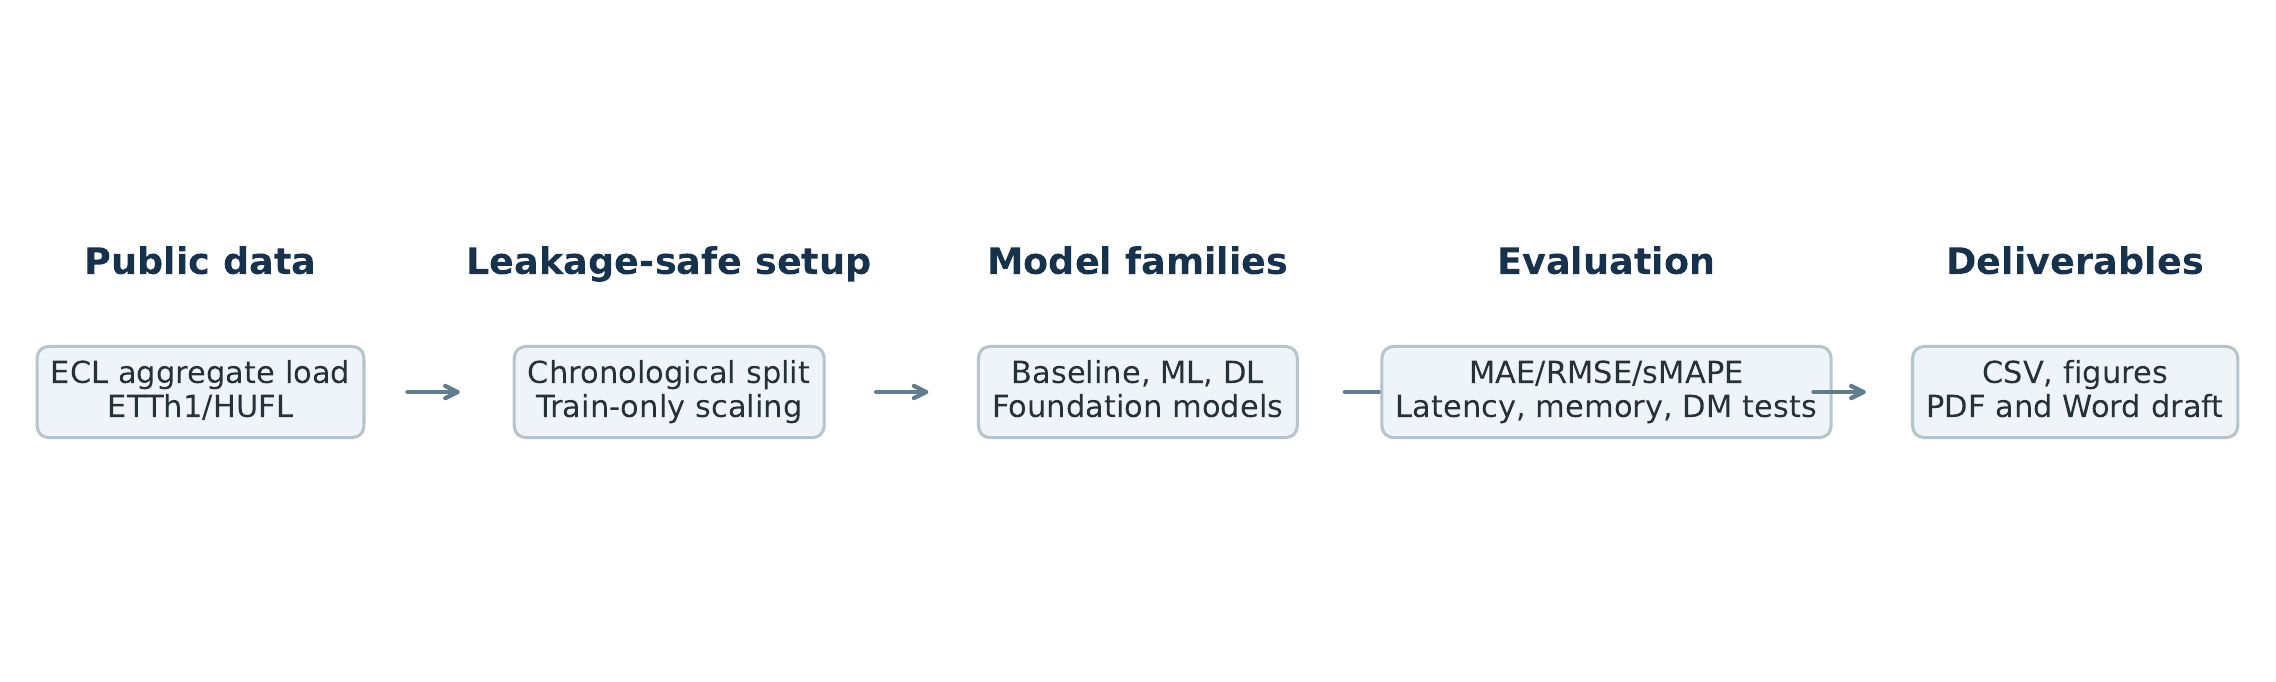
\includegraphics[width=6.6in,height=\textheight,keepaspectratio,alt={Figure 1. Experimental pipeline used for the benchmark.}]{docx_figures/fig1_methodology.png}
\caption{Figure 1. Experimental pipeline used for the benchmark.}
\end{figure}

\section{2. Related Work}\label{related-work}

Classical time-series forecasting methods, in particular ARIMA-family
models, remain important because they establish interpretable and
inexpensive references; automatic order selection by information
criteria such as AICc has made them practical to deploy on individual
series (Hyndman and Khandakar 2008). Machine-learning approaches based
on lagged targets, calendar variables, and gradient-boosted trees are
widely used in load forecasting because they are fast to train and
robust under tabular feature engineering (Chen and Guestrin 2016).

Deep-learning models such as LSTM (Hochreiter and Schmidhuber 1997),
attention-based architectures (Vaswani et al. 2017), Informer (Zhou et
al. 2021), DLinear (Zeng et al. 2023), PatchTST (Nie et al. 2023),
iTransformer (Liu et al. 2024), and TimesNet (Wu et al. 2023) have
broadened the long-horizon forecasting toolbox. Time-series foundation
models such as TimesFM (Das et al. 2024) and the Chronos family (Ansari
et al. 2024) motivate a new evaluation axis: no-task-specific-training
inference versus supervised training on the target dataset.

A fair comparison must state that public benchmarks may have appeared in
pretraining corpora. Therefore, zero-shot performance on ECL or ETT
should not be interpreted as guaranteed dataset-unseen generalization.
The narrower and reproducible claim in this work is that Chronos-Bolt
and TimesFM were run without task-specific training in this repository.

\section{3. Methodology}\label{methodology}

Given a univariate context window, the task is to predict the next H
observations for horizons H in \{24, 96, 168\}. The executed experiments
use a fixed context length of L=336 hours, which includes daily and
weekly seasonal information and permits use of lag-168 features.

The SeasonalNaive baseline repeats the most recent daily seasonal
pattern. The SARIMA baseline uses fixed-grid AICc selection on the
training split, then reuses the selected model on test windows via state
filtering rather than per-window refitting. XGBoost is trained as a
direct multi-output regressor using lag-1, lag-24, lag-168, rolling
means over 24 and 168 hours, and cyclic calendar features. DLinear,
PatchTST, and iTransformer are trained through NeuralForecast in the
same target-only setting, with a short validation-only learning-rate
sweep over 1e-3 and 5e-4 plus early stopping. Chronos-Bolt-Small and
TimesFM 2.5 are evaluated in zero-shot mode without task-specific
training.

All preprocessing for trained models is fitted only on the training
split, and metrics are computed after inverse-transforming predictions
to the original target scale. Foundation models and SARIMA are evaluated
directly on the original target scale.

\section{4. Experimental Setup}\label{experimental-setup}

The primary dataset is ECL, processed as aggregate hourly electricity
load across 321 clients. The secondary dataset is ETTh1 with HUFL as the
target. ETTh1 OT is oil temperature and is not used as electricity load.
ECL is split chronologically into 70\% train, 10\% validation, and 20\%
test. ETTh1 uses the standard 12-month, 4-month, 4-month chronological
split.

Accuracy is measured with MAE, RMSE, sMAPE, and wMAPE. Efficiency is
measured with training time, single-window inference latency (batch size
1), trainable parameters, and peak GPU memory. XGBoost, DLinear,
PatchTST, and iTransformer are evaluated across five seeds (42-46) and
reported as mean +/- standard deviation. SeasonalNaive, SARIMA,
Chronos-Bolt, and TimesFM are single-run deterministic or zero-shot
evaluations and are reported without across-seed standard deviation.

Diebold-Mariano tests are computed on per-window absolute errors for the
top two models by MAE at seed 42 for each dataset and horizon. Because
flattened point-wise MAE and per-window aggregation weight errors
differently, statistical-test rankings can differ slightly from table
rankings when models are very close.

\section{5. Results}\label{results}

\begin{figure}
\centering
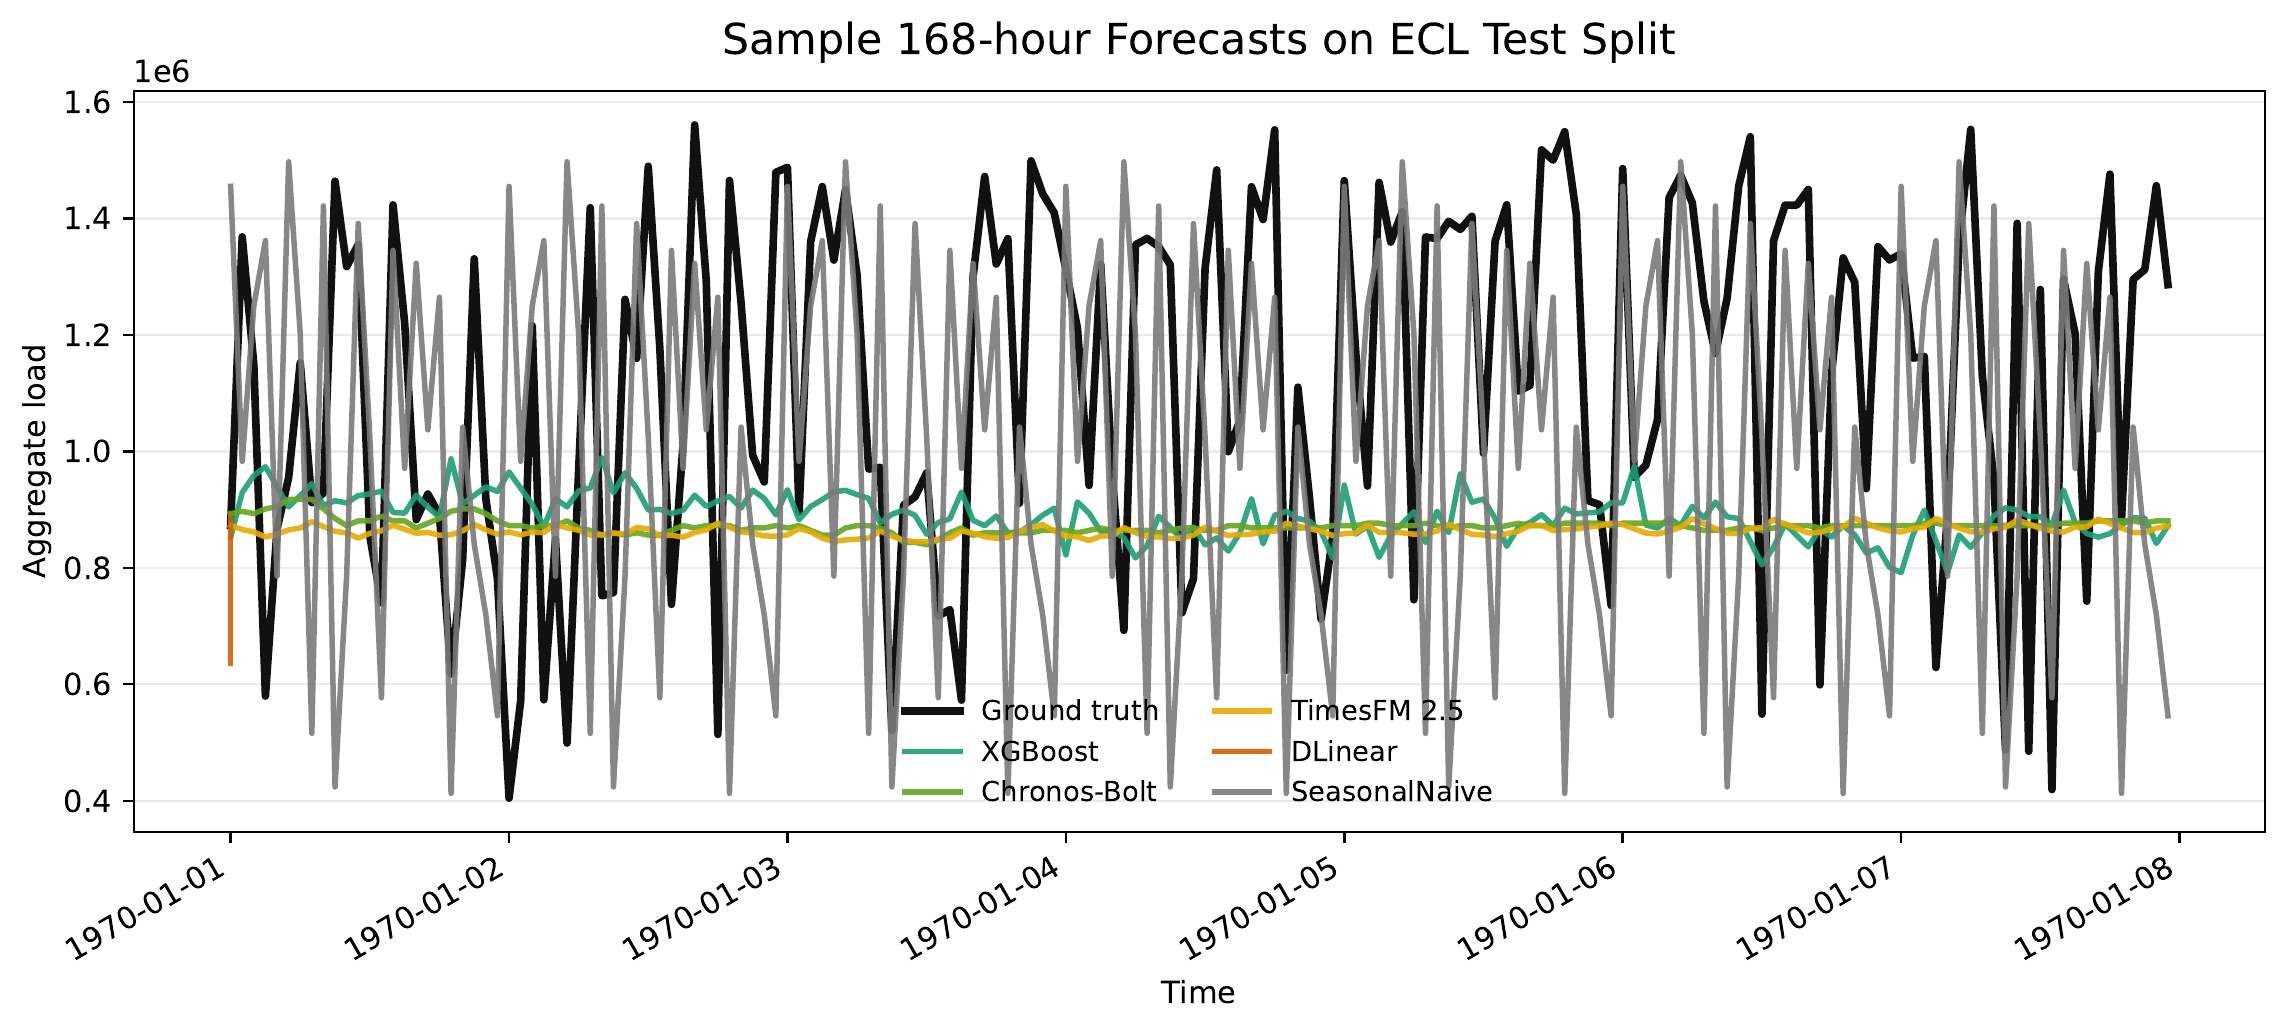
\includegraphics[width=6.6in,height=\textheight,keepaspectratio,alt={Figure 2. Sample 168 hour ECL forecasts from representative models.}]{docx_figures/fig2_forecasts.png}
\caption{Figure 2. Sample 168 hour ECL forecasts from representative
models.}
\end{figure}

\subsection{5.1 Accuracy on ECL}\label{accuracy-on-ecl}

On ECL, the strongest group consists of XGBoost and the two foundation
models. TimesFM has the lowest point-wise MAE at H=24, but the gap to
XGBoost and Chronos-Bolt is below 0.1\%, so the practical ranking among
the three is essentially flat at the shortest horizon. XGBoost is then
marginally best at H=96 and H=168, with Chronos-Bolt close at all three
horizons. The grid-tuned SARIMA tracks this top group within a small but
consistent gap and remains ahead of the trained neural models.

{\def\LTcaptype{none} % do not increment counter
\begin{longtable}[]{@{}
  >{\raggedright\arraybackslash}p{(\linewidth - 6\tabcolsep) * \real{0.2000}}
  >{\raggedleft\arraybackslash}p{(\linewidth - 6\tabcolsep) * \real{0.2667}}
  >{\raggedleft\arraybackslash}p{(\linewidth - 6\tabcolsep) * \real{0.2667}}
  >{\raggedleft\arraybackslash}p{(\linewidth - 6\tabcolsep) * \real{0.2667}}@{}}
\toprule\noalign{}
\begin{minipage}[b]{\linewidth}\raggedright
Model
\end{minipage} & \begin{minipage}[b]{\linewidth}\raggedleft
H=24 MAE
\end{minipage} & \begin{minipage}[b]{\linewidth}\raggedleft
H=96 MAE
\end{minipage} & \begin{minipage}[b]{\linewidth}\raggedleft
H=168 MAE
\end{minipage} \\
\midrule\noalign{}
\endhead
\bottomrule\noalign{}
\endlastfoot
TimesFM 2.5 & \textbf{259345.28} & 262766.32 & 265044.60 \\
Chronos-Bolt & 259546.11 & 262601.94 & 264268.27 \\
XGBoost & 259549.38 +/- 13.62 & \textbf{261792.58 +/- 9.36} &
\textbf{264220.96 +/- 24.77} \\
SARIMA & 263913.91 & 267033.48 & 271294.60 \\
DLinear & 278309.93 +/- 78.45 & 279227.54 +/- 52.48 & 280272.56 +/-
47.26 \\
PatchTST & 279295.35 +/- 274.56 & 280109.77 +/- 94.31 & 280876.20 +/-
109.22 \\
iTransformer & 283321.32 +/- 278.79 & 279842.21 +/- 148.37 & 279476.02
+/- 103.81 \\
SeasonalNaive & 338935.90 & 340658.82 & 343510.17 \\
\end{longtable}
}

\begin{figure}
\centering
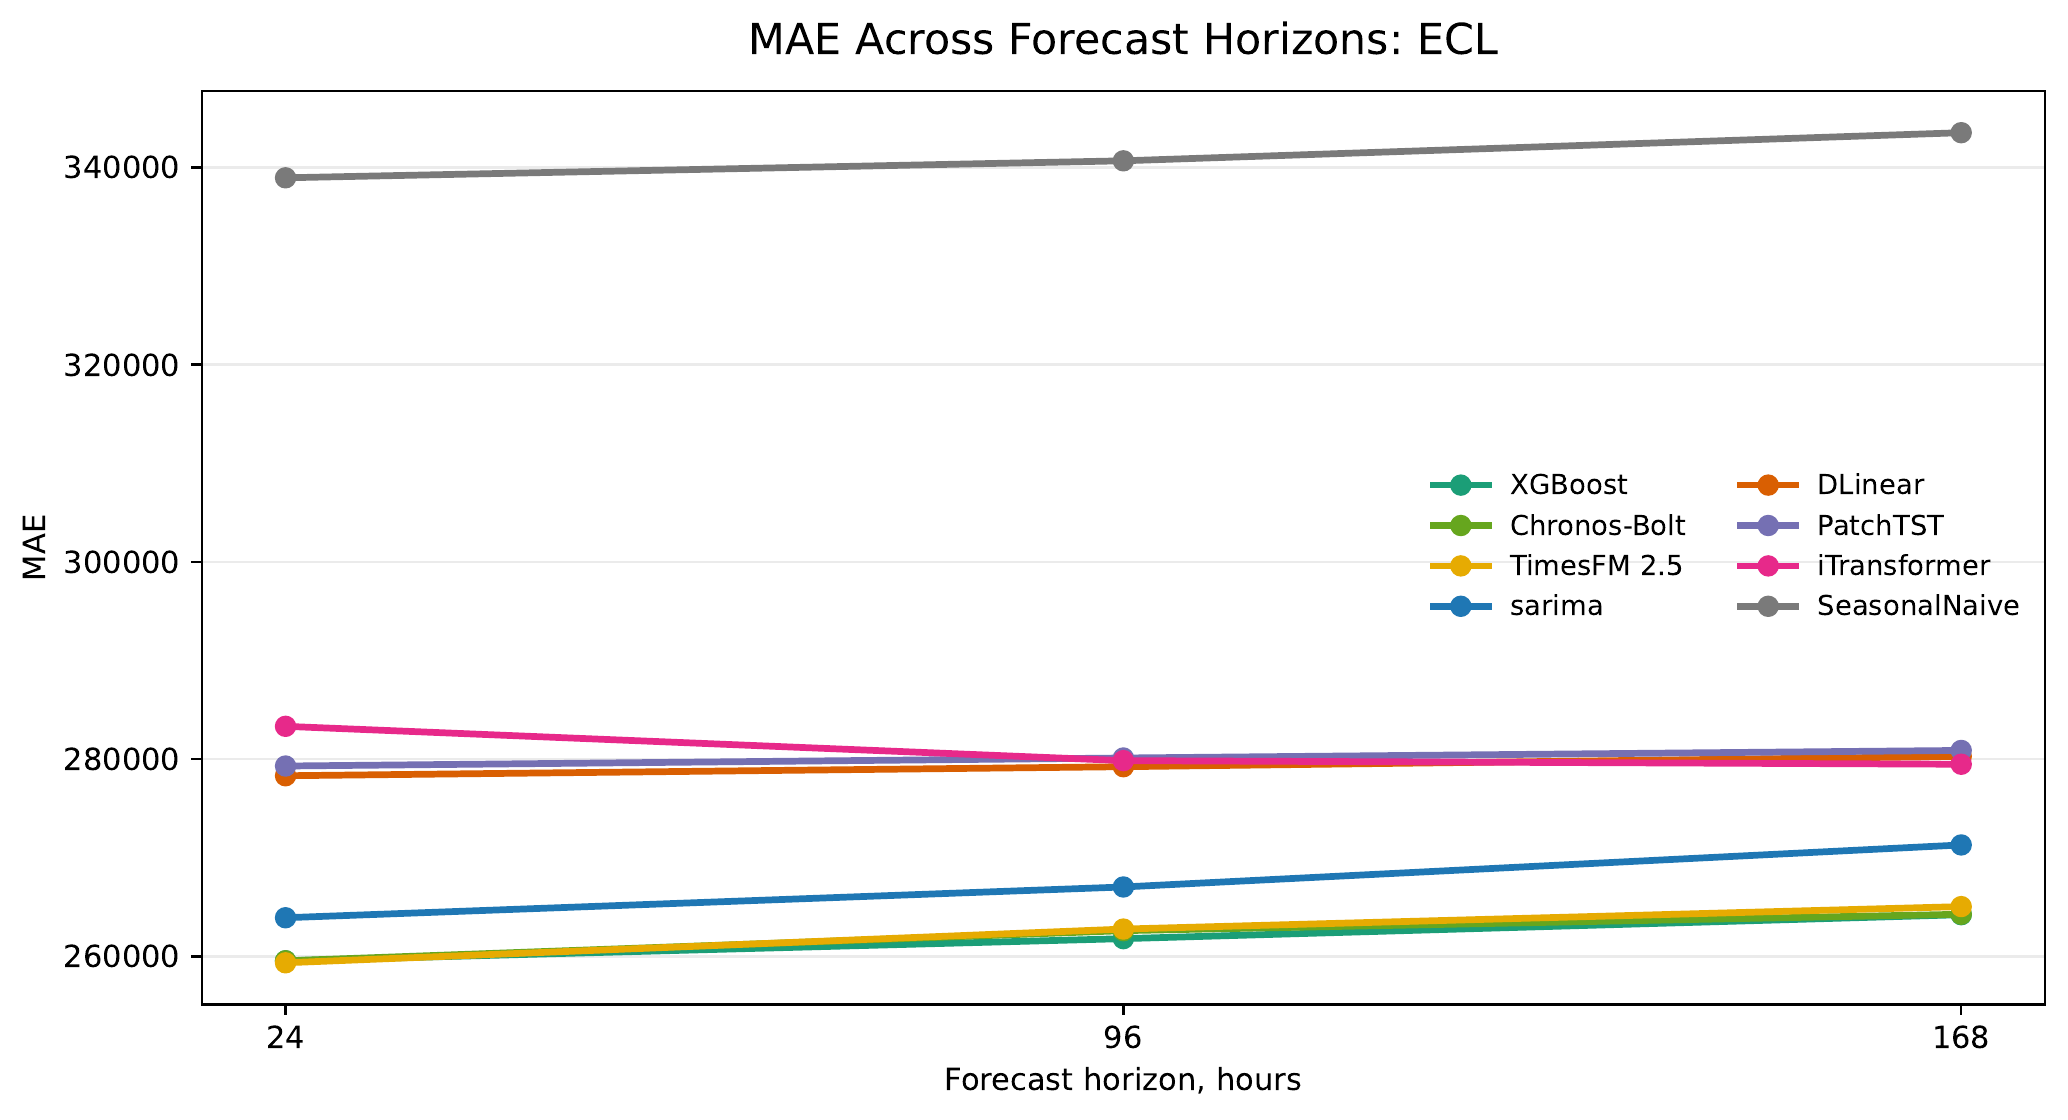
\includegraphics[width=6.6in,height=\textheight,keepaspectratio,alt={Figure 3. MAE across forecast horizons on ECL.}]{docx_figures/fig6_ecl_accuracy.png}
\caption{Figure 3. MAE across forecast horizons on ECL.}
\end{figure}

\subsection{5.2 Accuracy on ETTh1/HUFL}\label{accuracy-on-etth1hufl}

On ETTh1/HUFL, Chronos-Bolt is best at H=24. PatchTST is the strongest
trained model on the same horizon, while DLinear is best at H=96 and
H=168. TimesFM is competitive but not best on this benchmark. SARIMA is
close to the best classical baseline and beats XGBoost across all three
horizons, a role reversal versus ECL where XGBoost dominates SARIMA.

{\def\LTcaptype{none} % do not increment counter
\begin{longtable}[]{@{}lrrr@{}}
\toprule\noalign{}
Model & H=24 MAE & H=96 MAE & H=168 MAE \\
\midrule\noalign{}
\endhead
\bottomrule\noalign{}
\endlastfoot
Chronos-Bolt & \textbf{3.00} & 3.57 & 3.77 \\
PatchTST & 3.04 +/- 0.01 & 3.62 +/- 0.03 & 3.95 +/- 0.07 \\
DLinear & 3.08 +/- 0.00 & \textbf{3.55 +/- 0.00} & \textbf{3.70 +/-
0.00} \\
TimesFM 2.5 & 3.16 & 3.67 & 3.79 \\
iTransformer & 3.25 +/- 0.02 & 3.72 +/- 0.01 & 3.91 +/- 0.02 \\
SeasonalNaive & 3.31 & 3.92 & 4.18 \\
SARIMA & 3.45 & 3.90 & 4.18 \\
XGBoost & 3.89 +/- 0.01 & 4.21 +/- 0.01 & 4.27 +/- 0.01 \\
\end{longtable}
}

\begin{figure}
\centering
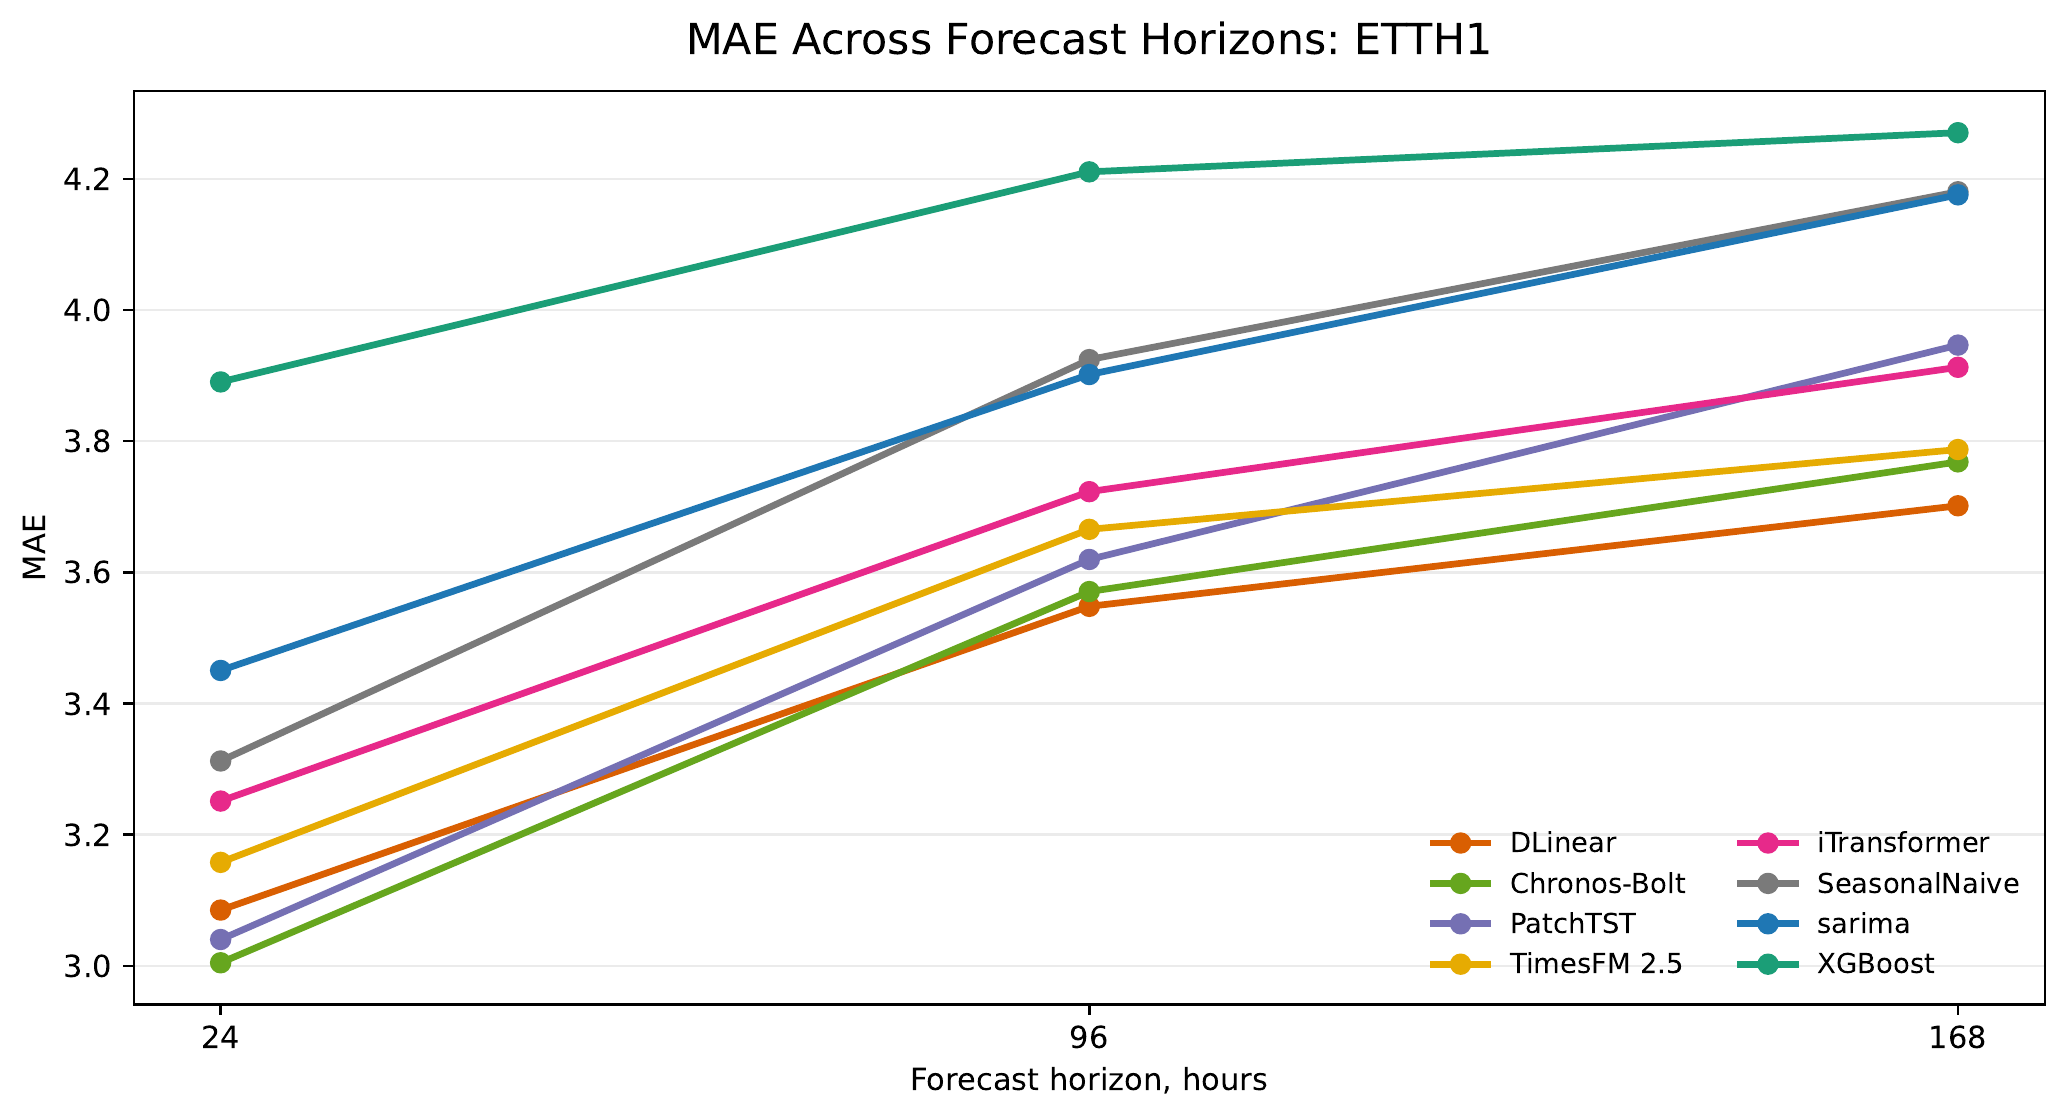
\includegraphics[width=6.6in,height=\textheight,keepaspectratio,alt={Figure 4. MAE across forecast horizons on ETTh1/HUFL.}]{docx_figures/fig7_etth1_accuracy.png}
\caption{Figure 4. MAE across forecast horizons on ETTh1/HUFL.}
\end{figure}

\subsection{5.3 Cross-Dataset View}\label{cross-dataset-view}

The normalized heatmap emphasizes that the best model family changes
with dataset and horizon. On ECL, XGBoost and the two foundation models
form a tight group. On ETTh1/HUFL, Chronos-Bolt and DLinear dominate
different horizons. The winner summary provides the same conclusion in a
more compact form.

\begin{figure}
\centering
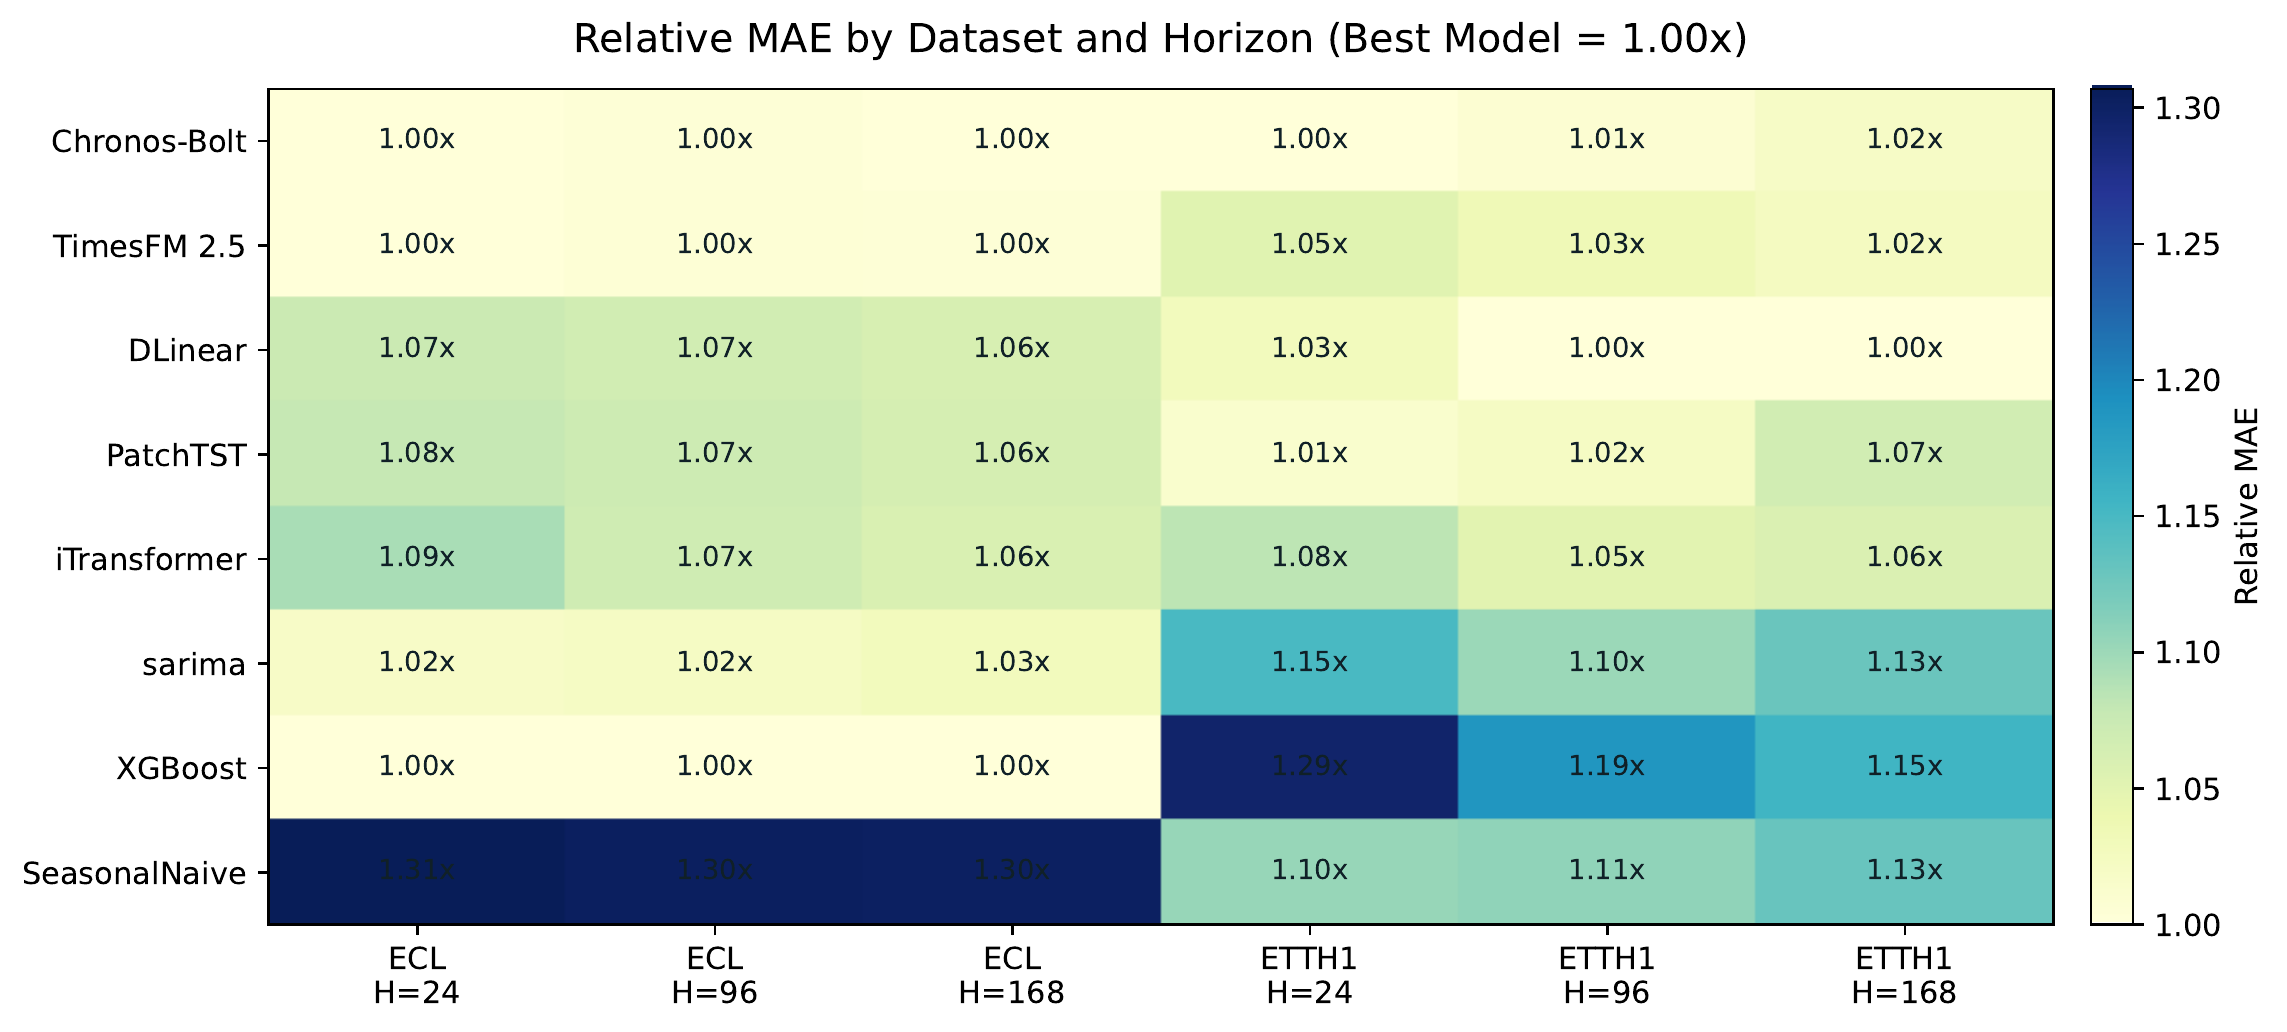
\includegraphics[width=6.6in,height=\textheight,keepaspectratio,alt={Figure 5. Relative MAE heatmap across datasets and horizons. Values are normalized within each dataset-horizon pair; the best model is 1.00x.}]{docx_figures/fig3_heatmap.png}
\caption{Figure 5. Relative MAE heatmap across datasets and horizons.
Values are normalized within each dataset-horizon pair; the best model
is 1.00x.}
\end{figure}

\begin{figure}
\centering
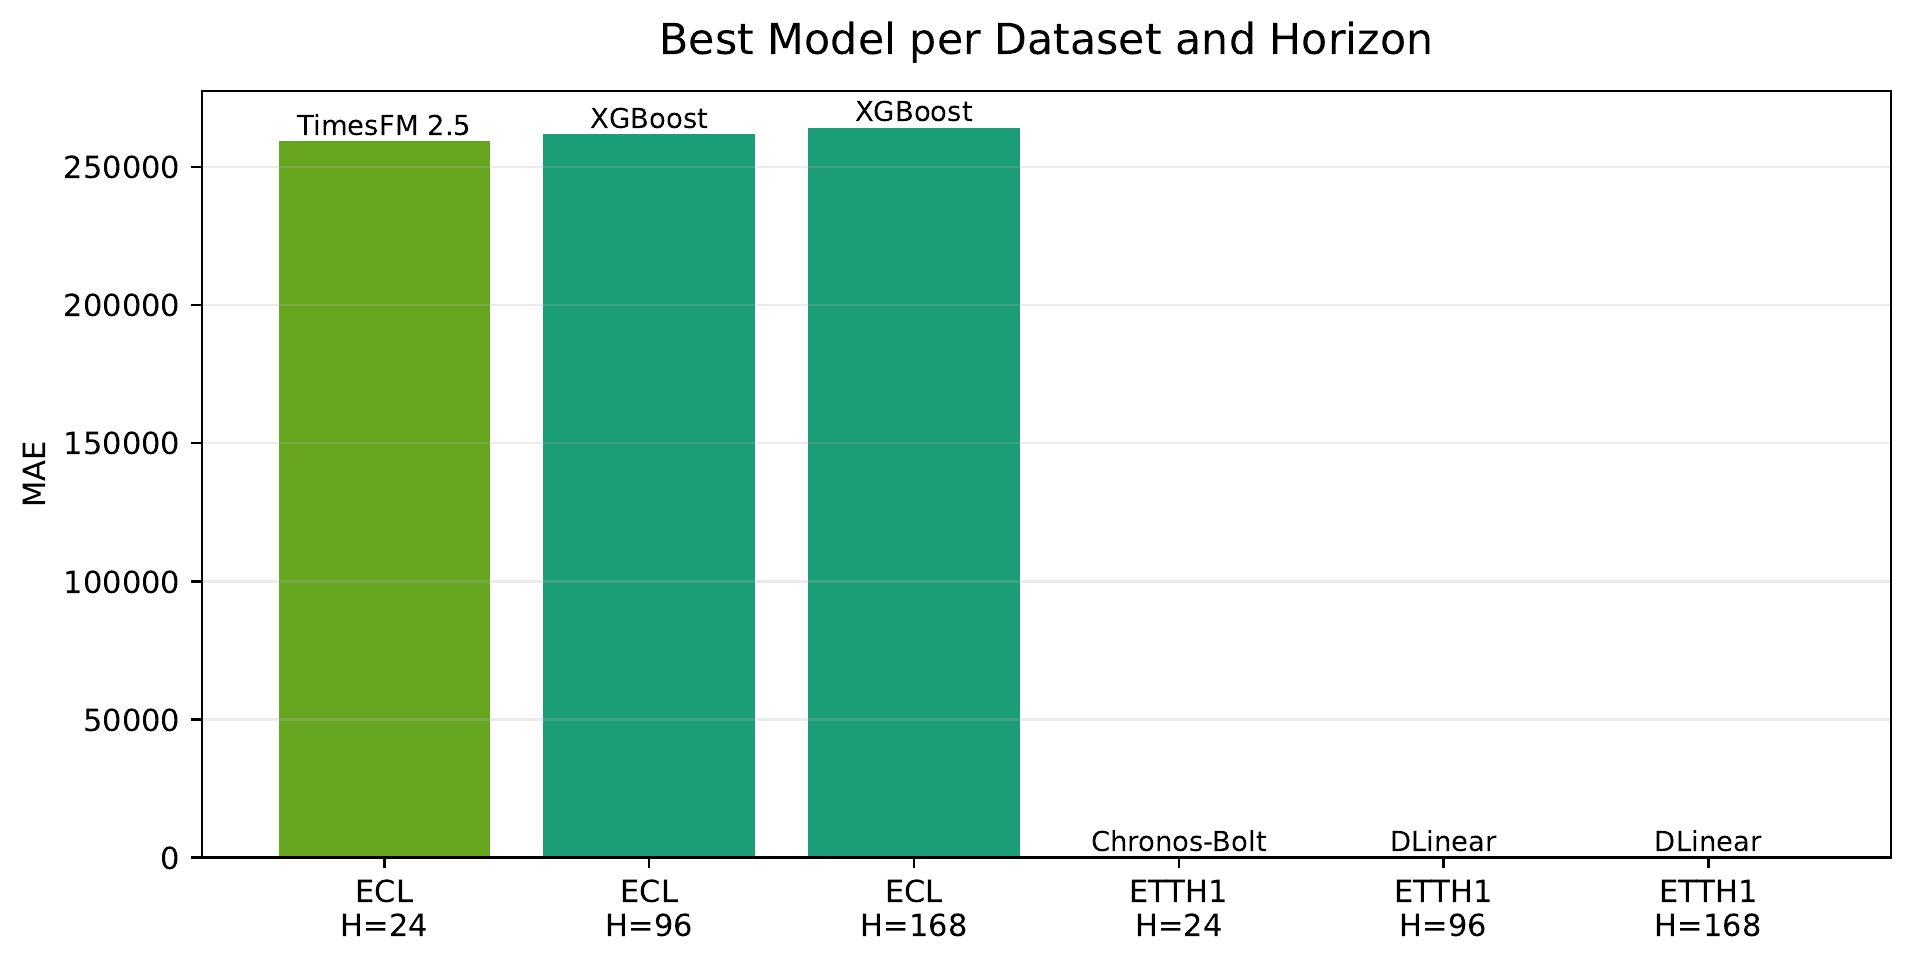
\includegraphics[width=5.8in,height=\textheight,keepaspectratio,alt={Figure 6. Best model per dataset and horizon.}]{docx_figures/fig5_horizon.png}
\caption{Figure 6. Best model per dataset and horizon.}
\end{figure}

\subsection{5.4 Efficiency and Statistical
Tests}\label{efficiency-and-statistical-tests}

The efficiency results show the deployment trade-off. SeasonalNaive and
SARIMA have the lowest inference latencies. XGBoost remains faster than
the neural and TimesFM models and does not require GPU inference.
Chronos-Bolt is competitive for zero-shot inference, while TimesFM has
the highest latency and GPU memory use in this implementation.

{\def\LTcaptype{none} % do not increment counter
\begin{longtable}[]{@{}llrrr@{}}
\toprule\noalign{}
Dataset / H=96 & Model & MAE & Inference ms/window & GPU MB \\
\midrule\noalign{}
\endhead
\bottomrule\noalign{}
\endlastfoot
ECL & XGBoost & 261792.58 & 25.09 & 0.0 \\
ECL & Chronos-Bolt & 262601.94 & 39.64 & 345.8 \\
ECL & TimesFM 2.5 & 262766.32 & 91.99 & 895.6 \\
ETTh1/HUFL & DLinear & 3.55 & 39.29 & 29.8 \\
ETTh1/HUFL & Chronos-Bolt & 3.57 & 36.24 & 345.8 \\
ETTh1/HUFL & XGBoost & 4.21 & 24.47 & 0.0 \\
\end{longtable}
}

\begin{figure}
\centering
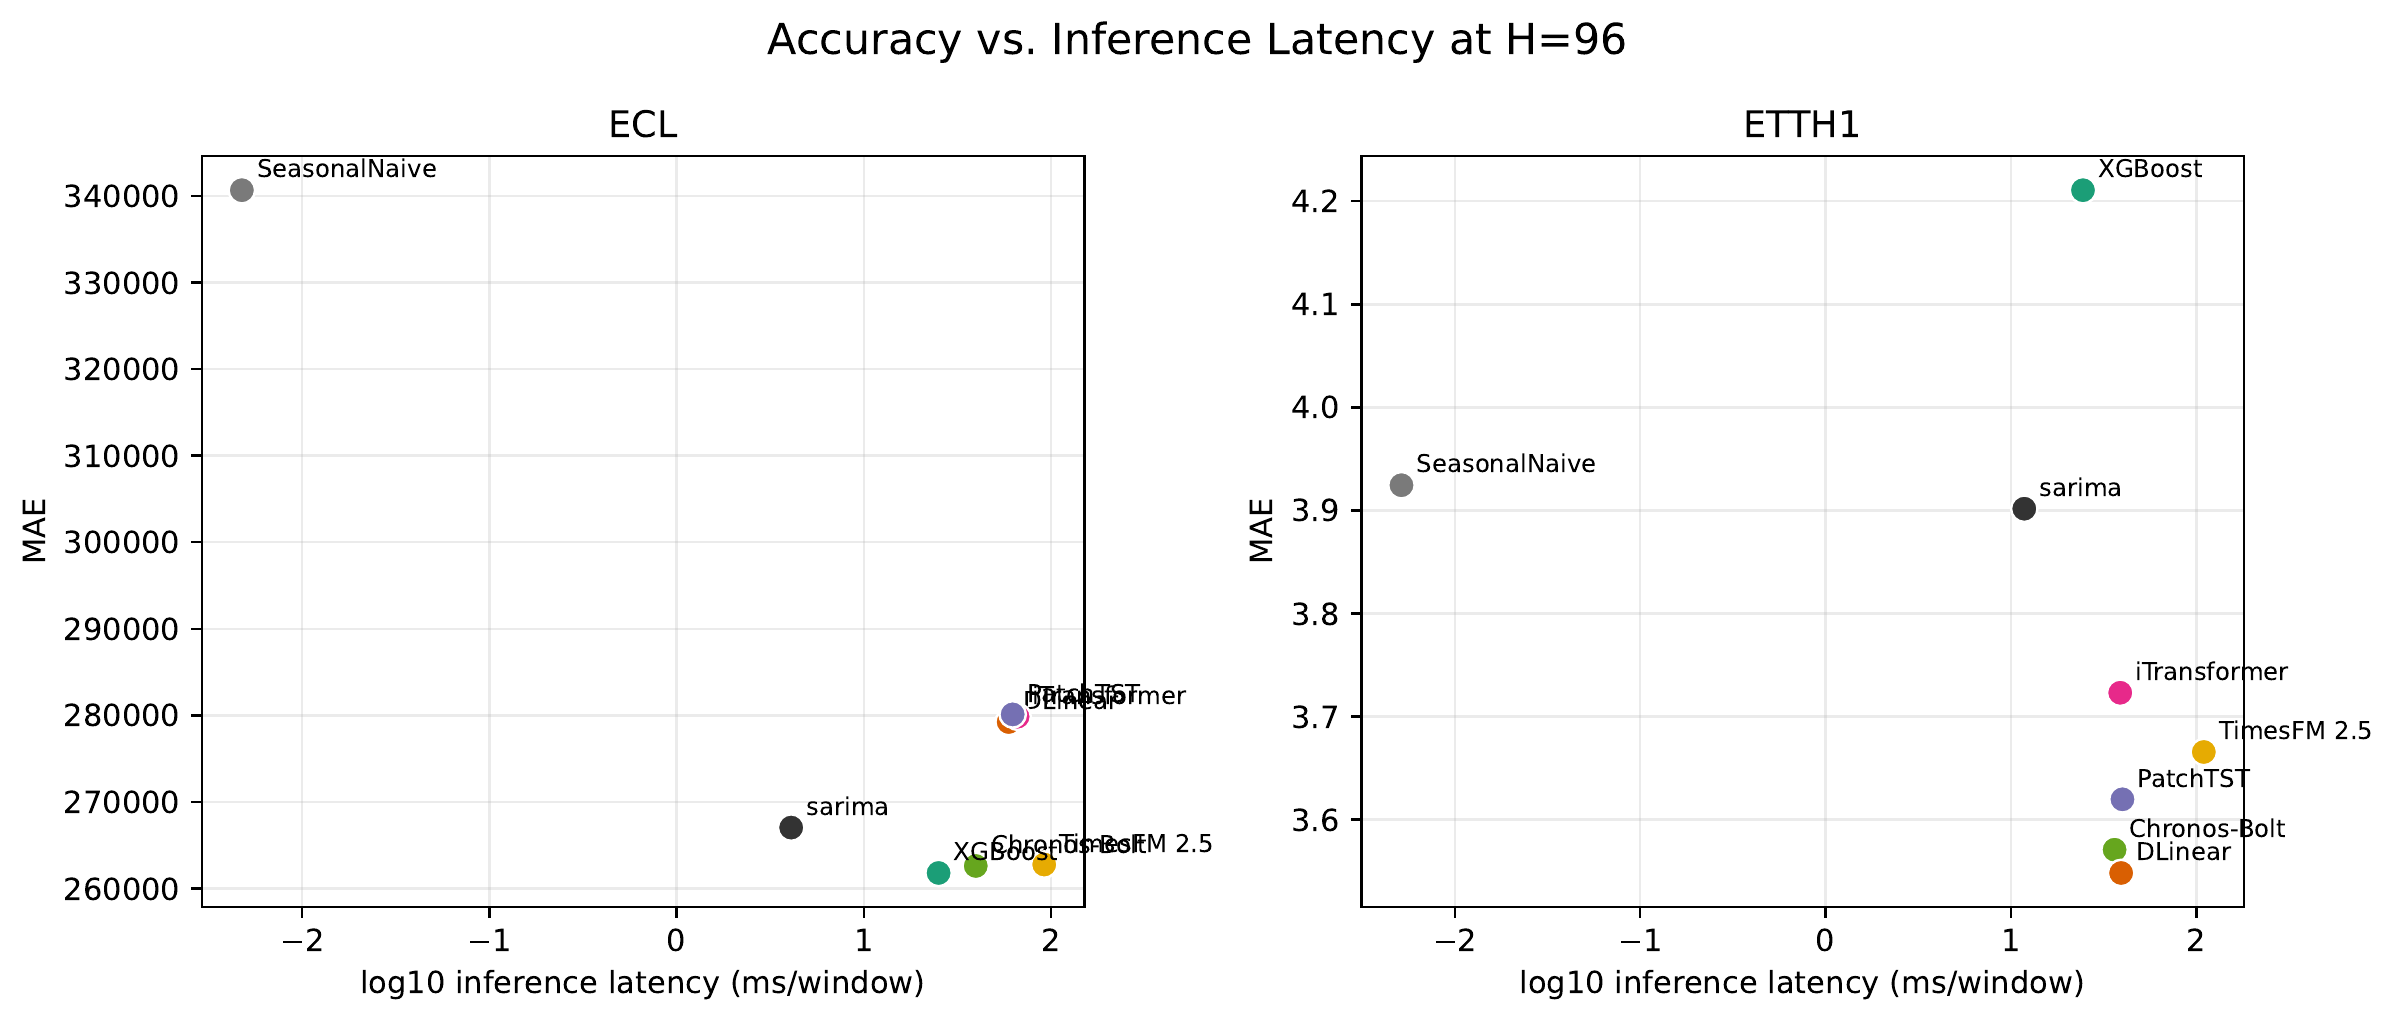
\includegraphics[width=6.6in,height=\textheight,keepaspectratio,alt={Figure 7. Accuracy-latency view at H=96.}]{docx_figures/fig4_pareto.png}
\caption{Figure 7. Accuracy-latency view at H=96.}
\end{figure}

The Diebold-Mariano tests confirm that the top comparisons are not only
small numerical differences in flattened MAE. On ECL, the H=96 and H=168
results favor XGBoost over Chronos-Bolt. At H=24, TimesFM and XGBoost
are nearly tied in operational terms even though the test rejects equal
predictive accuracy. On ETTh1/HUFL, the tests support Chronos-Bolt at
H=24 and DLinear at the two longer horizons.

{\def\LTcaptype{none} % do not increment counter
\begin{longtable}[]{@{}llrrl@{}}
\toprule\noalign{}
Dataset / Horizon & Comparison & Statistic & p-value & Significant \\
\midrule\noalign{}
\endhead
\bottomrule\noalign{}
\endlastfoot
ECL / H=24 & TimesFM vs XGBoost & 13.45 & \textless0.001 & Yes \\
ECL / H=96 & XGBoost vs Chronos-Bolt & -38.15 & \textless0.001 & Yes \\
ECL / H=168 & XGBoost vs Chronos-Bolt & -2.88 & 0.004 & Yes \\
ETTh1 / H=24 & Chronos-Bolt vs PatchTST & -3.39 & \textless0.001 &
Yes \\
ETTh1 / H=96 & DLinear vs Chronos-Bolt & -2.48 & 0.013 & Yes \\
ETTh1 / H=168 & DLinear vs Chronos-Bolt & -8.81 & \textless0.001 &
Yes \\
\end{longtable}
}

\section{6. Discussion}\label{discussion}

The results show that model choice is dataset-dependent. On aggregate
ECL load, engineered lag features with XGBoost remain an extremely
strong and inexpensive option. The grid-tuned SARIMA baseline is also
competitive and remains ahead of the trained neural architectures
evaluated here. Foundation models are attractive when avoiding
task-specific training is valuable: Chronos-Bolt is close to XGBoost on
ECL and best at the shortest ETTh1/HUFL horizon. DLinear is the
strongest trained neural model in this benchmark and dominates the
longer ETTh1/HUFL horizons.

From a deployment perspective, the models occupy different operating
regimes. XGBoost is the most attractive choice when a conventional
supervised training pipeline is acceptable: it is accurate on ECL, has
low single-window latency, and does not require GPU inference. SARIMA is
a competitive low-cost backup with no learned features and millisecond
inference. Chronos-Bolt is useful when task-specific training is
undesirable, for example in cold-start industrial monitoring, rapid
prototyping, or sites where historical data cannot be pooled for model
training. TimesFM shows strong point accuracy at the shortest ECL
horizon, but its latency is substantially higher in this implementation.

The transformer results should be read carefully. PatchTST and
iTransformer are credible architectures, but this benchmark uses a
compact target-only configuration and a fixed training budget. Their
underperformance here does not imply that transformers are generally
unsuitable for load forecasting; rather, it shows that they do not
automatically beat simpler methods under constrained, reproducible
settings.

\section{7. Limitations}\label{limitations}

The main limitations are public-benchmark pretraining-contamination risk
for foundation models, limited hyperparameter search, target-only
modeling, and the absence of private industrial deployment data. A
rolling AutoARIMA baseline was attempted, but full per-origin grid
search was prohibitively expensive in this protocol. The partial run is
retained in repository logs but excluded from the main comparison
tables. The grid-tuned SARIMA reported here is the practical
replacement: orders are selected on the training split by AICc and the
parameters are reused for forecast windows, giving a fast and
well-defined ARIMA-family baseline.

Chronos-Bolt also emits a warning that prediction lengths above 64 are
outside its recommended range. Therefore, H=96 and H=168 Chronos results
should be interpreted as practical stress tests rather than optimal use
of that model. The foundation-model results should also not be
overinterpreted as guaranteed dataset-unseen zero-shot generalization.
ECL and ETT are public benchmarks and may overlap with pretraining or
evaluation corpora used during model development.

\section{8. Conclusion}\label{conclusion}

We built and executed a reproducible STLF benchmark pipeline on ECL and
ETTh1/HUFL. On ECL, XGBoost, Chronos-Bolt, and TimesFM are operationally
near-tied across horizons, with TimesFM best at H=24 and XGBoost best at
H=96 and H=168. On ETTh1/HUFL, Chronos-Bolt wins H=24, PatchTST is the
best trained model at H=24, and DLinear wins H=96 and H=168. These
findings support a pragmatic recommendation: compare against strong
simple baselines first, use DLinear and PatchTST as neural references,
and treat foundation models as valuable cold-start tools rather than
universally dominant replacements for supervised forecasting.

\section*{References}\label{references}
\addcontentsline{toc}{section}{References}

\protect\phantomsection\label{refs}
\begin{CSLReferences}{1}{1}
\bibitem[\citeproctext]{ref-ansari2024chronos}
Ansari, Abdul Fatir, Lorenzo Stella, Caner Turkmen, et al. 2024.
{``Chronos: Learning the Language of Time Series.''} \emph{Transactions
on Machine Learning Research}. \url{https://arxiv.org/abs/2403.07815}.

\bibitem[\citeproctext]{ref-chen2016xgboost}
Chen, Tianqi, and Carlos Guestrin. 2016. {``XGBoost: A Scalable Tree
Boosting System.''} \emph{Proceedings of the 22nd ACM SIGKDD
International Conference on Knowledge Discovery and Data Mining},
785--94. \url{https://doi.org/10.1145/2939672.2939785}.

\bibitem[\citeproctext]{ref-das2024timesfm}
Das, Abhimanyu, Weihao Kong, Rajat Sen, and Yichen Zhou. 2024. {``A
Decoder-Only Foundation Model for Time-Series Forecasting.''}
\emph{International Conference on Machine Learning}.
\url{https://arxiv.org/abs/2310.10688}.

\bibitem[\citeproctext]{ref-hochreiter1997lstm}
Hochreiter, Sepp, and Jürgen Schmidhuber. 1997. {``Long Short-Term
Memory.''} \emph{Neural Computation} 9 (8): 1735--80.
\url{https://doi.org/10.1162/neco.1997.9.8.1735}.

\bibitem[\citeproctext]{ref-hyndman2008automatic}
Hyndman, Rob J., and Yeasmin Khandakar. 2008. {``Automatic Time Series
Forecasting: The Forecast Package for r.''} \emph{Journal of Statistical
Software} 27 (3): 1--22. \url{https://doi.org/10.18637/jss.v027.i03}.

\bibitem[\citeproctext]{ref-liu2024itransformer}
Liu, Yong, Tengge Hu, Haoran Zhang, et al. 2024. {``iTransformer:
Inverted Transformers Are Effective for Time Series Forecasting.''}
\emph{International Conference on Learning Representations}.
\url{https://arxiv.org/abs/2310.06625}.

\bibitem[\citeproctext]{ref-nie2023patchtst}
Nie, Yuqi, Nam H. Nguyen, Phanwadee Sinthong, and Jayant Kalagnanam.
2023. {``A Time Series Is Worth 64 Words: Long-Term Forecasting with
Transformers.''} \emph{International Conference on Learning
Representations}. \url{https://arxiv.org/abs/2211.14730}.

\bibitem[\citeproctext]{ref-vaswani2017attention}
Vaswani, Ashish, Noam Shazeer, Niki Parmar, et al. 2017. {``Attention Is
All You Need.''} \emph{Advances in Neural Information Processing
Systems}. \url{https://arxiv.org/abs/1706.03762}.

\bibitem[\citeproctext]{ref-wu2023timesnet}
Wu, Haixu, Tengge Hu, Yong Liu, Hang Zhou, Jianmin Wang, and Mingsheng
Long. 2023. {``TimesNet: Temporal 2D-Variation Modeling for General Time
Series Analysis.''} \emph{International Conference on Learning
Representations}. \url{https://arxiv.org/abs/2210.02186}.

\bibitem[\citeproctext]{ref-zeng2023dlinear}
Zeng, Ailing, Muxi Chen, Lei Zhang, and Qiang Xu. 2023. {``Are
Transformers Effective for Time Series Forecasting?''} \emph{Proceedings
of the AAAI Conference on Artificial Intelligence}.
\url{https://arxiv.org/abs/2205.13504}.

\bibitem[\citeproctext]{ref-zhou2021informer}
Zhou, Haoyi, Shanghang Zhang, Jieqi Peng, et al. 2021. {``Informer:
Beyond Efficient Transformer for Long Sequence Time-Series
Forecasting.''} \emph{Proceedings of the AAAI Conference on Artificial
Intelligence}. \url{https://arxiv.org/abs/2012.07436}.

\end{CSLReferences}
